\documentclass[a4paper,11pt, notitlepage ]{article}
\usepackage[T1]{fontenc}
\usepackage[polish]{babel}
\usepackage[utf8]{inputenc}
\usepackage{lmodern}
\usepackage{enumitem}
\usepackage{indentfirst}
\usepackage{graphicx}
\usepackage{wrapfig}
\usepackage{fancyhdr}
\usepackage{lastpage}
\pagestyle{fancy}
\fancyhf{}
\setcounter{page}{1}
\rfoot{Strona \thepage \hspace{1pt} z \pageref{LastPage}}
\selectlanguage{polish}
\makeatletter
\newcommand{\linia}{\rule{\linewidth}{0.4mm}}
\renewcommand{\maketitle}{\begin{titlepage}
    \vspace*{1cm}
    \begin{center}\small
    Politechnika Warszawska\\
    Wydział Elektryczny
    \end{center}
    \vspace{3cm}
    \noindent\linia
    \begin{center}
      \LARGE \textsc{\@title}
         \end{center}
     \linia
    \vspace{0.5cm}
    \begin{flushright}
    \begin{minipage}{8cm}
    \textit{\small Autorzy:}\\
    \normalsize \textsc{\@author} \par
    \end{minipage}
    \end{flushright}
    \vspace*{\stretch{6}}
    \begin{center}
    \@date
    \end{center}
  \end{titlepage}%
}
\makeatother
\author{J.~Korczakowski, nr albumu 291079\\ B.~Suchocki, nr albumu 291111\\ Grupa projektowa nr 11}
\title{Specyfikacja implementacyjna symulatora automatu komórkowego \textsl{Wireworld}}
\frenchspacing
\begin{document}
\maketitle
\setcounter{page}{2}
\tableofcontents
\newpage

\section{Diagram klas}
\begin{figure}[h]
\centering
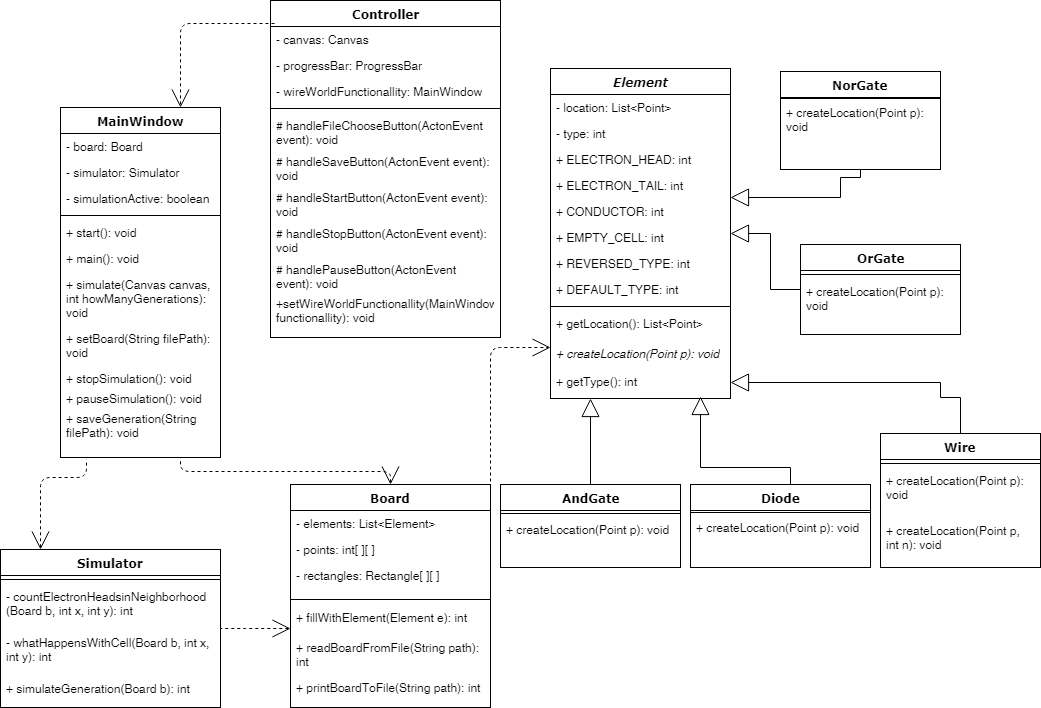
\includegraphics[width=13cm]{ClassDiagram}
\caption{Diagram klas}
\end{figure}

\section{Opis klas}

\subsection{Simulator}
Odpowiada za symulację kolejnych generacji komórek.


Pola: \verb+brak+.

Metody:
\begin{enumerate}
\item \verb+private int countElectronHeadsInNeighbourhood(Board b, int x,+ \verb+int y)+.
\begin{itemize}
\item Argumenty:
\begin{itemize}
\item \verb+b+  - obiekt klasy \verb+Board+ reprezentujący bieżący stan generacji komórek,
\item \verb+x,y+ - współrzędne komórki, dla której zliczana jest ilość sąsiadujących z nią \verb+głów elektronu+.
\end{itemize}
\item Wartość zwracana:
\begin{itemize}
\item Ilość \verb+głów elektronu+ sąsiadujących z daną komórką.
\end{itemize}
\item Działanie:
\begin{itemize}
\item Funkcja zlicza ilość \verb+głów elektronu+ w sąsiedztwie komórki o podanym położeniu według zasad sąsiedztwa Moore'a.
\end{itemize}
\end{itemize}	

\item \begin{verbatim}private int whatHappensWithCell(Board b, int x, int y). \end{verbatim}
\begin{itemize}
\item Argumenty:
\begin{itemize}
\item \verb+b+  - obiekt klasy \verb+Board+ reprezentujący bieżący stan generacji komórek,
\item \verb+x,y+ - współrzędne komórki, dla której ustalany jest nowy stan.
\end{itemize}
\item Wartość zwracana:
\begin{itemize}
\item Liczba (stała) określająca nowy stan analizowanej komórki.
\end{itemize}
\item Działanie:
\begin{itemize}
\item Funkcja, korzystając z funkcji \verb+countElectronHeadsInNeigh-+ \verb+bourhood+ określa czy, w następnej generacji, będzie \verb+głową+ \verb+elektronu+, \verb+ogonem elektronu+, \verb+przewodnikiem+ czy \verb+pustą+ \verb+komórką+. Dla każdego z takich stanów zwraca liczbę całkowitą (stałą) go symbolizującą. Odpowiednio: \verb+ELECTRON_HEAD+, \verb+ELECTRON_TAIL+, \verb+CONDUCTOR+, \verb+EMPTY_CELL+.
\end{itemize}
\end{itemize}


\item \verb+public int simulateGeneration(Board b)+.
\begin{itemize}
\item Argumenty:
\begin{itemize}
\item \verb+b+  - obiekt klasy \verb+Board+ reprezentujący bieżący stan generacji komórek,
\end{itemize}
\item Wartość zwracana:
\begin{itemize}
\item Liczba całkowita okrelająca czy symulacja zakończyła się powodzeniem (0 - jeśli tak, 1 - jeśli nie).
\end{itemize}
\item Działanie:
\begin{itemize}
\item Metoda symuluje przejście komórek do następnej generacji. Symulacja wykonywana jest poprzez iteracyjne sprawdzanie poprzedniego stanu analizowanej komórki oraz zliczanie (przy użyciu funkcji \verb+countElectronHeadsInNeighbourhood+) \verb+głów+ \verb+elektronu+ w jej sąsiedztwie . Na podstawie tej analizy (przy użyciu metody \verb+whatHappensWithCell+ nastąpi określenie, do jakiego stanu przejdzie dana komórka. W wyniku działania metody, zmodyfikowany zostanie obiekt b przekazany jako argument jej wywołania. Po zakończeniu działania metody, będzie on przechowywać stan aktualnej generacji (po symulacji).
\end{itemize}
\end{itemize}



\end{enumerate}

\subsection{Controller}
Odpowiada za odpowiadanie na akcje użytkownika (np. wciśnięcie przycisku). 

Pola:
\begin{itemize}
\item \verb+private Canvas canvas+ - graficzna reprezentacja planszy,
\item \verb+private ProgressBar progressBar+ pasek wizualizujący postęp symulacji,
\item \verb+private MainWindow wireWorldFunctionallity+ - obiekt potrzebny do używania funkcjonalności automatu WireWorld w odpowiedzi na akcje użytkownika.
\end{itemize}

Metody:

\begin{enumerate}

\item \verb+public void setWireWorldFunctionallity(MainWindow+ \\ \verb+functionallity)+
\begin{itemize}
\item Argumenty:
\begin{itemize}
\item \verb+functionallity+ - obiekt klasy MainWindow umożliwiający korzystanie z funkcjonalności automatu WireWorld w odpowiedzi na akcje użytkownika.
\end{itemize}
\item Wartość zwracana:
\begin{itemize}
\item Void
\end{itemize}
\item Działanie:
\begin{itemize}
\item Metoda ustawia pole wireWorldFunctionallity na argument wywołania.
\end{itemize}
\end{itemize}


\item \begin{verbatim}protected void handleFileChooseButton(ActionEvent event). \end{verbatim}
\begin{itemize}
\item Argumenty:
\begin{itemize}
\item \verb+event+ - obiekt klasy \verb+ActionEvent+ reprezentujący zdarzenie naciśnięcia przycisku.
\end{itemize}
\item Wartość zwracana:
\begin{itemize}
\item Void
\end{itemize}
\item Działanie:
\begin{itemize}
\item Metoda, w odpowiedzi na naciśnięcie przycisku wyboru pliku weściowego przez użytkownika, wyświetla dialog, w którym użytkownik może wybrać plik wejściowy z odpowiedniej lokalizacji. Po wyborze, ścieżka do pliku wświetlona zostaje w+polu poniżej przycisku i wywołana zostaje metoda \verb+setBoard+ obiektu klasy MainWindow (jako argument wywołania, przekazywana jest lokalizacja pliku wejściowego).
\end{itemize}
\end{itemize}


\item \begin{verbatim} protected void handleStartButton(ActionEvent event). \end{verbatim}
\begin{itemize}
\item Argumenty:
\begin{itemize}
\item \verb+event+ - obiekt klasy \verb+ActionEvent+ reprezentujący zdarzenie naciśnięcia przycisku.
\end{itemize}
\item Wartość zwracana:
\begin{itemize}
\item Void
\end{itemize}
\item Działanie:
\begin{itemize}
\item Metoda, w odpowiedzi na naciśnięcie przycisku startu przez użytkownika, wywołuję metodę \verb+simulate+ obiektu klasy MainWindow.
\end{itemize}
\end{itemize}


\item \begin{verbatim}protected void handleStopButton(ActionEvent event). \end{verbatim}
\begin{itemize}
\item Argumenty:
\begin{itemize}
\item \verb+event+ - obiekt klasy \verb+ActionEvent+ reprezentujący zdarzenie naciśnięcia przycisku.
\end{itemize}
\item Wartość zwracana:
\begin{itemize}
\item Void
\end{itemize}
\item Działanie:
\begin{itemize}
\item Metoda, w odpowiedzi na naciśnięcie przycisku stopu przez użytkownika, wywołuje metodę \verb+stopSimulation+ obiektu klasy MainWindow.
\end{itemize}
\end{itemize}


\item \begin{verbatim}protected void handlePauseButton(ActionEvent event). \end{verbatim}
\begin{itemize}
\item Argumenty:
\begin{itemize}
\item \verb+event+ - obiekt klasy \verb+ActionEvent+ reprezentujący zdarzenie naciśnięcia przycisku.
\end{itemize}
\item Wartość zwracana:
\begin{itemize}
\item Void
\end{itemize}
\item Działanie:
\begin{itemize}
\item Metoda, w odpowiedzi na naciśnięcie przycisku pauzy przez użytkownika, wywołuje metodę \verb+pauseSimulation+ obiektu klasy MainWindow.
\end{itemize}
\end{itemize}


\item \begin{verbatim}protected void handleSaveButton(ActionEvent event). \end{verbatim}
\begin{itemize}
\item Argumenty:
\begin{itemize}
\item \verb+event+ - obiekt klasy \verb+ActionEvent+ reprezentujący zdarzenie naciśnięcia przycisku.
\end{itemize}
\item Wartość zwracana:
\begin{itemize}
\item Void
\end{itemize}
\item Działanie:
\begin{itemize}
\item Metoda, w odpowiedzi na naciśnięcie przycisku zapisu przez użytkownika, wyświetla dialog umożliwiający wybranie ścieżki do pliku wyjściowego oraz uruchamia metodę \verb+saveGeneration+ obiektu klasy MainWindow, przekazując lokalizację pliku jako argument wywołania.
\end{itemize}
\end{itemize}




\end{enumerate}

\subsection{MainWindow}
Jest modułem realizującym wszystkie funkcjonalności automatu komórkowego \verb+WireWorld+.

Pola:
\begin{itemize}
\item \verb+private Board board+ - obiekt przechowujący stan kolejnych generacji,
\item \verb+private Simulator simulator+ obiekt umożliwiający symulację kolejnych generacji,
\item \verb+private boolean simulationActive+ - zmienna służąca monitorowaniu czy wątek przeprowadzający kolejne symulacje powinien zakończyć działanie.
\end{itemize}

Metody:

\begin{enumerate}
\item \begin{verbatim}public void start(). \end{verbatim}
\begin{itemize}
\item Argumenty: \verb+brak+.
\item Wartość zwracana:
\begin{itemize}
\item Void
\end{itemize}
\item Działanie:
\begin{itemize}
\item Metoda inicjalizuje pola klasy oraz wyświetla graficzny interfejs użytkownika.
\end{itemize}
\end{itemize}


\item \begin{verbatim} public static void main(String[] args). \end{verbatim}
\begin{itemize}
\item Argumenty:
\begin{itemize}
\item \verb+args+ - ewentualne argumenty wywołania programu (jeśli program uruchomiony został z wiersza poleceń).
\end{itemize}
\item Wartość zwracana:
\begin{itemize}
\item Void
\end{itemize}
\item Działanie:
\begin{itemize}
\item Metoda uruchamia metodę \verb+start+.
\end{itemize}
\end{itemize}



\item \begin{verbatim}public void simulate(Canvas canvas, int howManyGenerations). \end{verbatim}
\begin{itemize}
\item Argumenty:
\begin{itemize}
\item \verb+canvas+ - obiekt klasy \verb+Canvas+ reprezentujący graficzny wygląd planszy,
\item \verb+howManyGenerations+ - liczba całkowita określające liczbę symulacji do przeprowadzenia.
\end{itemize}
\item Wartość zwracana:
\begin{itemize}
\item Void
\end{itemize}
\item Działanie:
\begin{itemize}
\item Metoda przeprowadza kolejne symulacje przejścia komórek do następnej generacji (korzystając z metody \verb+simulateGeneration+ obiektu klasy Simulator. Każdą kolejną generację wyświetla na graficznej planszy.
\end{itemize}
\end{itemize}


\item \begin{verbatim}public void setBoard(String filePath). \end{verbatim}
\begin{itemize}
\item Argumenty:
\begin{itemize}
\item \verb+filePath+ - lokalizacja pliku wejściowego.
\end{itemize}
\item Wartość zwracana:
\begin{itemize}
\item Void
\end{itemize}
\item Działanie:
\begin{itemize}
\item Metoda ustawia zawartość pola \verb+board+ na podstawie pliku wejściowego, korzystając z metody \verb+readBoardFromFile+ klasy Board.
\end{itemize}
\end{itemize}

\item \begin{verbatim}public void stopSimulation(). \end{verbatim}
\begin{itemize}
\item Argumenty: \verb+brak+.
\item Wartość zwracana:
\begin{itemize}
\item Void
\end{itemize}
\item Działanie:
\begin{itemize}
\item Metoda kończy wcześniej rozpoczętą symulację ustawiając wartość zmiennej \verb+simulationActive+ na \verb+false+ oraz przywraca początkowy stan generacji.
\end{itemize}
\end{itemize}


\item \begin{verbatim}public void pauseSimulation(). \end{verbatim}
\begin{itemize}
\item Argumenty: \verb+brak+.
\item Wartość zwracana:
\begin{itemize}
\item Void
\end{itemize}
\item Działanie:
\begin{itemize}
\item Metoda zatrzymuje wcześniej rozpoczętą symulację ustawiając wartość zmiennej \verb+simulationActive+ na \verb+false+ .
\end{itemize}
\end{itemize}


\item \begin{verbatim}public void saveGeneration(String filePath). \end{verbatim}
\begin{itemize}
\item Argumenty:
\begin{itemize}
\item \verb+filePath+ - lokalizacja pliku wyjściowego, do którego zapisany będzie stan bieżącej generacji.
\end{itemize}
\item Wartość zwracana:
\begin{itemize}
\item Void
\end{itemize}
\item Działanie:
\begin{itemize}
\item Metoda zapisuje (korzystając z metody \verb+printBoardToFile+ obiektu klasy Board) stan bieżącej generacji do pliku, którego lokalizacją jest argument wywołania metody.
\end{itemize}
\end{itemize}




\end{enumerate}



\subsection{Element}
Klasa abstrakcyjna opisująca pojedynczy element obwodu \textsl{Wireworld}. Dziedziczą po niej klasy, które opisują poszczególne typy obwodu.

Pola:
\begin{itemize}
\item \verb+private List<Point> location+ - zawiera listę punktów
zajmowanych przez daną strukturę.
\item \verb+private int type+ - zawiera informację czy dana struktura jest odwrócona, czy znajduje się w domyślnym położeniu
\item \verb+public static final int ELECTRON_HEAD+ - zawiera stałą oznaczającą głowę elektronu.
\item \verb+public static final int ELECTRON_TAIL+ - zawiera stałą oznaczającą ogon elektronu.
\item \verb+public static final int CONDUCTOR+ - zawiera stałą oznaczającą przewodnik.
\item \verb+public static final int EMPTY_CELL+ - zawiera stałą oznaczającą pustą komórkę.
\item \verb+public static final int REVERSED_TYPE+ - zawiera stałą oznaczającą odwrócone położenie.
\item \verb+public static final int DEDAULT_TYPE+ - zawiera stałą oznaczającą domyślne położenie. 
\end{itemize}

Metody:
\begin{enumerate}
\item \verb+public List<Point> getLocation()+.
\begin{itemize}
\item Argumenty:
\item Wartość zwracana:
\begin{itemize}
\item Lista zawierająca punkty(\verb+List<Point>+).
\end{itemize}
\item Działanie:
\begin{itemize}
\item Jest to metoda dostępowa zwracająca listę punktów, które zajmuje dany element.
\end{itemize}
\end{itemize}

\item \verb+public abstract void createLocation( Point p )+.
\begin{itemize}
\item Argumenty:
\begin{itemize}
\item \verb+p+ - Punkt początkowy elementu.
\end{itemize}
\item Wartość zwracana:
\begin{itemize}
\item \verb+Void+
\end{itemize}
\item Działanie:
\end{itemize}


\item \verb+public int getType()+.
\begin{itemize}
\item Argumenty:
\item Wartość zwracana:
\begin{itemize}
\item Typ elementu.
\end{itemize}
\item Działanie:
\begin{itemize}
\item Jest to metoda dostępowa zwracająca typ elementu.
\end{itemize}
\end{itemize}
\end{enumerate}

\subsection{AndGate}
Klasa dziedzicząca po klasie \verb+Element+. Opisuje strukturę odpowiadającą bramce logicznej AND.

\begin{enumerate}
\item \verb+public void createLocation( Point p )+.
\begin{itemize}
\item Argumenty:
\begin{itemize}
\item \verb+p+ - Punkt początkowy elementu.
\end{itemize}
\item Wartość zwracana:
\begin{itemize}
\item \verb+Void+
\end{itemize}
\item Działanie:
\begin{itemize}
\item Metoda po otrzymaniu punktu początkowego wypełnia pole \verb+location+ punktami, które zajmuje bramka logiczna AND.
\end{itemize}
\end{itemize}
\end{enumerate}

\subsection{OrGate}
Klasa dziedzicząca po klasie \verb+Element+. Opisuje strukturę odpowiadającą bramce logicznej OR.

\begin{enumerate}
\item \verb+public void createLocation( Point p )+.
\begin{itemize}
\item Argumenty:
\begin{itemize}
\item \verb+p+ - Punkt początkowy elementu.
\end{itemize}
\item Wartość zwracana:
\begin{itemize}
\item \verb+Void+
\end{itemize}
\item Działanie:
\begin{itemize}
\item Metoda po otrzymaniu punktu początkowego wypełnia pole \verb+location+ punktami, które zajmuje bramka logiczna OR.
\end{itemize}
\end{itemize}
\end{enumerate}

\subsection{NorGate}
Klasa dziedzicząca po klasie \verb+Element+. Opisuje strukturę odpowiadającą bramce logicznej NOR.

\begin{enumerate}
\item \verb+public void createLocation( Point p )+.
\begin{itemize}
\item Argumenty:
\begin{itemize}
\item \verb+p+ - Punkt początkowy elementu.
\end{itemize}
\item Wartość zwracana:
\begin{itemize}
\item \verb+Void+
\end{itemize}
\item Działanie:
\begin{itemize}
\item Metoda po otrzymaniu punktu początkowego wypełnia pole \verb+location+ punktami, które zajmuje bramka logiczna NOR.
\end{itemize}
\end{itemize}
\end{enumerate}

\subsection{Diode}
Klasa dziedzicząca po klasie \verb+Element+. Opisuje strukturę odpowiadającą diodzie.

\begin{enumerate}
\item \verb+public void createLocation( Point p )+.
\begin{itemize}
\item Argumenty:
\begin{itemize}
\item \verb+p+ - Punkt początkowy elementu.
\end{itemize}
\item Wartość zwracana:
\begin{itemize}
\item \verb+Void+
\end{itemize}
\item Działanie:
\begin{itemize}
\item Metoda po otrzymaniu punktu początkowego wypełnia pole \verb+location+ punktami, które zajmuje dioda.
\end{itemize}
\end{itemize}
\end{enumerate}




\subsection{Wire}
Klasa dziedzicząca po klasie \verb+Element+. Opisuje strukturę odpowiadającą kablowi.

\begin{enumerate}
\item \verb+public void createLocation( Point p )+.
\begin{itemize}
\item Argumenty:
\begin{itemize}
\item \verb+p+ - Punkt początkowy elementu.
\end{itemize}
\item Wartość zwracana:
\begin{itemize}
\item \verb+Void+
\end{itemize}
\item Działanie:
\begin{itemize}
\item Metoda po otrzymaniu punktu początkowego wypełnia pole \verb+location+ punktami, które zajmuje kabel o długości domyślnej 2.
\end{itemize}
\end{itemize}

\item \verb+public void createLocation( Point p, int n )+.
\begin{itemize}
\item Argumenty:
\begin{itemize}
\item \verb+p+ - Punkt początkowy elementu.
\item \verb+n+ - Długość kabla.
\end{itemize}
\item Wartość zwracana:
\begin{itemize}
\item \verb+Void+
\end{itemize}
\item Działanie:
\begin{itemize}
\item Metoda po otrzymaniu punktu początkowego wypełnia pole \verb+location+ punktami, które zajmuje kabel o podanej długości \verb+n+.
\end{itemize}
\end{itemize}
\end{enumerate}

\subsection{Board}
Klasa obsługująca planszę. Umożliwia odczytanie planszy z pliku, zapis do pliku i wypełnienie planszy elementami.

Pola:
\begin{enumerate}
\item \verb+private List<Elements> elements+ - lista zawierająca wszystkie elementy z podanego pliku.
\item \verb+private int [][] points+ - dwuwymiarowa tablica zawierająca stany poszczególnych komórek wyrażone za pomocą liczb całkowitych.
\item \verb+private Rectangle [][] rectangles+ - dwuwymiarowa tablica kwadratów zawierająca graficzną reprezentację stanów komórek. 
\end{enumerate}

Metody:
\begin{enumerate}
\item \verb+public int readBoardFromFile(String path)+.
\begin{itemize}
\item Argumenty:
\begin{itemize}
\item \verb+path+ - ścieżka do pliku z którego chcemy odczytać elementy.
\end{itemize}
\item Wartość zwracana:
\begin{itemize}
\item Wartość liczbowa odpowiadająca sukcesowi lub porażce podczas wczytywania z pliku.
\end{itemize}
\item Działanie:
\begin{itemize}
\item Metoda odczytuje z wybranego przez użytkownika z pliku po kolei elementy obwodu. W przypadku błędnego elementu metoda go pominie. Metoda podczas wczytywania uzupełnia listę elementów \verb+elements+.
\end{itemize}
\end{itemize}


\item \verb+public int fillWithElement+.
\begin{itemize}
\item Argumenty:
\begin{itemize}
\item \verb+e+ - element, który ma zostać wpisany do tablic \verb+points+ i \verb+rectangles+.
\end{itemize}
\item Wartość zwracana:
\begin{itemize}
\item Wartość liczbowa odpowiadająca sukcesowi lub porażce podczas wypełniania tablic.
\end{itemize}
\item Działanie:
\begin{itemize}
\item Metoda wypełnia tablice \verb+points+ i \verb+rectangles+ punktami danego elementu.
\end{itemize}
\end{itemize}

\item \verb+public int printBoardToFile(String path)+.
\begin{itemize}
\item Argumenty:
\begin{itemize}
\item \verb+path+ - ścieżka pliku, do którego ma być zapisana lista elementów.
\end{itemize}
\item Wartość zwracana:
\begin{itemize}
\item Wartość liczbowa odpowiadająca sukcesowi lub porażce podczas zapisywania.
\end{itemize}
\item Działanie:
\begin{itemize}
\item Metoda tworzy na podstawie tablicy \verb+points+ listę elementów i zapisuje ją do wybranego pliku.
\end{itemize}
\end{itemize}


\end{enumerate}


\section{Testy}
Podczas implementacji projektu wykonamy testy jednostkowe dla modułów \verb+Board+ oraz \verb+Simulator+. Klasy testujące nazwiemy BoardTest oraz SimulatorTest, nazwy metod testujących będą wskazywać jednoznacznie jaką funkcjonalność/przypadek poddamy sprawdzeniu. Do wykonania testów jednostkowych użyjemy bibliotek \verb+JUnit+, \verb+AssertJ+ oraz \verb+Mockito+.
Pozostałe moduły przetestujemy uruchamiając program i obserwując jego zachowanie.


\section{Ekrany programu}
Ekran naszego programu został przedstawiony w specyfikacji funkcjonalnej w rozdziale 4.3 Ekrany działania programu.

\section{Strona techniczna projektu}
\begin{description}
\item[Wersja języka] \hfill \\
W naszym projekcie będziemy korzystać z języka Java w wersji 8. Chcemy używać wersji 8, ponieważ do budowy GUI użyjemy technologii JavaFX, która została w wersji 8 ulepszona i poprawiona.
\item[Używany system operacyjny]\hfill \\
 Projekt będzie tworzony w systemie Windows.
\item[Dodatkowe narzędzia]\hfill \\
Potrzebne biblioteki (\verb+JUnit+, \verb+AssertJ+, \verb+Mockito+) dołączymy do programu używając narzędzia \verb+Maven+.
\item[Wersjonowanie]\hfill \\
Podczas tworzenia projektu będziemy go wersjonować zaczynając od \verb+0.1+, a gotowa wersja naszego programu będzie miała numer \verb+1.0+. Podczas pracy z Gitem będziemy tworzyć nowy branch za każdym razem gdy będziemy chcieli wprowadzić nową funkcjonalność.
\end{description}

\end{document}